\chapter{Metodología} \label{chap:metod}

%%%%%%%%%%%%%%%%%%%%%%%%%%%%%%%%%%%%%%%%%%%%%%%%%%%%%%%%%%%%%%%
% Presentación del apartado y reportar la estructura
%%%%%%%%%%%%%%%%%%%%%%%%%%%%%%%%%%%%%%%%%%%%%%%%%%%%%%%%%%%%%%%
Este apartado detalla la metodología seguida en el trabajo. Se estructura como sigue: la primera sección lista los objetivos generales y específicos. La segunda describe las distintas fuentes de datos consideradas; la disponibilidad de datos influye en las decisiones de diseño tomadas más adelante. Las siguientes secciones describen los objetivos específicos en detalle; elección del modelo, construcción de la matriz de tiempos de residencia y uso de Filtro de Kalman en la estimación de parámetros.


%%%%%%%%%%%%%%%%%%%%%%%%%%%%%%%%%%%%%%%%%%%%%%%%%%%%%%%%%%%%%%
% Aqui solo voy a divagar c/r a lo que necesito hacer 
%%%%%%%%%%%%%%%%%%%%%%%%%%%%%%%%%%%%%%%%%%%%%%%%%%%%%%%%%%%%%%
% \begin{itemize}
%     \item Cuando trate el modelo completo (con clases y todo eso), los casos detectados pueden no ser la mejor opción para ajustar el modelo. La trazabilidad y la velocidad de detección en las clases bajas es menor que en clases altas (ellos tienen resultados mucho más rápidos). La cantidad de fallecidos, sin embargo, es un dato mucho más certero, el DEIS ha hecho un buen trabajo en saber quiénes han fallecido de covid. Según Mena, en los fallecidos además se nota la desigualdad, en el hecho que el exceso de muertes en jóvenes de clases sociales más bajas es mucho mayor. Creo que no hay problema en usar los fallecidos como observación... siempre y cuando las tasas sean conocidas y no por estimar, en ese caso creo que perdería la observabilidad.
    
    
%     \item Esto debería llevarme a replantear el modelo que estoy usando, debo considerar los muertos, y es posible que los hospitalizados también sean una buena fuente de información. Pero esto deja la duda de cómo ordenar los compartimientos para infección. Debería considerar expuestos, supongo, y la mayoría separa sintomáticos de asintomáticos. El problema más grande que sigo teniendo y que me molesta, es el hecho de que estoy necesitando demasiados parámetros, y que para fijarlos probablemente no haré pooling (o bien terminaré haciendo pooling total). Estoy segura que alguna estrategia de pooling parcial sería maravilloso, pero no sabría hacerla. Además creo que esto no es tan necesario, creo que debería revisar otras publicaciones con modelos multiclases para ver cómo lo enfrentan. 
    
    
%     \item Aun no tengo idea cómo fijar los riesgos. Definitivamente hay que hacer un análisis de sensibilidad (averiguar cómo), y aún no tengo claro si en la bibliografía se ha usado el modelo con ambientes (y no patches, que es el que sí usan). Creo que debo dedicar una sección a este estudio. No solo está el tema de los riesgos, también qué ambientes elijo, porque tampoco es claro, tenemos hartos, y podrían ser menos. Creo que sería bueno hacer un modelo de juguete con dos o tres ambientes, y ver qué pasa.
    
%     \item Cómo actualizar la matriz de tiempos de residencia. Este es por lejos el problema que más me molesta, porque Cattarina tiene razón, y los datos del plan paso a paso no capturan bien las diferencias (y está probado en varios artículos que las comunas de menor nivel socioeconómico disminuyen mucho menos su movilidad). Probablemente debería hacer algún tipo de análisis de sensibilidad aquí también, pero nuevamente no sé cómo. Me tinca que el ensamble de hecho funcionaría bien para eso, ver todas las posibles trayectorias. El problema con ensamble es que no tengo idea qué hacer con la distribución inicial, y cómo elegir bien las matrices de ruido, aunque había algunos artículos al respecto. 
% \end{itemize}


% Además aún no defino bien qué es lo que quiero hacer con esta cosa. Qué estoy tratando de hacer con KF? Averiguar un parámetro? Hasta ahora lo quiero usar para averiguar la tasa de contagio, que es un valor variable. Así que el paper de máx verosimilitud parece ser adecuado. Pero la controlabilidad es lo que me tiene con problemas. Creo que debería considerar el R efectivo, se puede calcular teóricamente y tal vez comparar con los que les dan en la página.

%%%%%%%%%%%%%%%%%%%%%%%%%%%%%%%%%%%%%%%%%%%%%%%%%%%%%%%%%%%%%%%
% Índice 
%%%%%%%%%%%%%%%%%%%%%%%%%%%%%%%%%%%%%%%%%%%%%%%%%%%%%%%%%%%%%%%

% Plantear objetivos generales y específicos, preguntas que guían la investigación. 

\section{Datos disponibles}\label{sec:datos-disp}

Esta sección describe las distintas fuentes de datos consideradas en el estudio. Los datos de interés pueden ser clasificados en tres categorías. En primer lugar, se busca caracterizar a la población de la Región Metropolitana, en términos etarios y socioeconómicos. Esto se logra mediante el Censo 2017 \ref{sec:censo} y el Índice de Prioridad Social 2019 \ref{sec:ips}.

En segundo lugar, se quiere conocer el comportamiento de la población, específicamente su uso del tiempo. La relación entre viajes y tiempos de actividad es utilizada en varios modelos \cite{Kitamura1988}\cite{Axhausen1992} y aprovechada para obtener información de encuestas de viajes como la Origen-Destino \cite{Munizaga2011}. En esa dirección, se considera la Encuesta Origen Destino Santiago 2012, descrita en la sección \ref{sec:eod}, ya que es una fuente bastante rica; provee información muy granular de personas, viajes y sus propósitos. Datos más actualizados que capturan las variaciones debido a la pandemia son los Informes de Movilidad Local sobre COVID-19, presentados en la sección \ref{sec:google}, y el Uso de infraestructura de telecomunicaciones, en la sección \ref{data:isci}.

Finalmente, se requieren datos para entender el avance de la pandemia en la Región Metropolitana. Datos-COVID19, un repositorio \cite{MINCIENCIA} mantenido por la Mesa de Datos del Ministerio de Ciencia, Tecnología, Conocimiento e Innovación, contiene distintas series de tiempo de casos confirmados, hospitalizados, fallecidos, vacunados en el país, con distintos niveles de agregación. Se comenta en más detalle en la sección \ref{sec:datos-minsal}.

% Para cada base de datos: 
% - Institución que la recopila 
% - Resumen de la metodología 
% - Datos que contiene 
% - Algunos resultados que sean relevantes para el trabajo 
% - Datos que sean de particular interés

%\noindent \textbf{Censo 2017}
\subsection{Censo 2017}\label{sec:censo}

El Censo de Población y Vivienda 2017 fue un proceso liderado por el Instituto Nacional de Estadística (INE), y permitió contar y caracterizar a 17.574.003 personas y 6.499.355 viviendas en todo el territorio nacional.
% Podría definir aquí zona censal, lo usan la EOD y los de movilidad del ISCI.

Para el levantamiento del Censo del año 2017 y la desagregación de los datos censales se utiliza en primer lugar la División Política Administrativa del país; regiones y comunas. Luego, el territorio de cada comuna se divide en distritos censales, los que pueden ser urbanos, rurales o mixtos. A su vez, en el área urbana se reconocen zonas censales, las que están compuestas de manzanas, y en el área rural, localidades.

El Censo está disponible en \url{http://www.censo2017.cl/}. Los datos de interés son la población de la Región Metropolitana, desagregada por zona censal o comuna, sexo y edad.


%\noindent \textbf{\'Indice de prioridad social (IPS) 2019}
\subsection{\'Indice de prioridad social (IPS) 2019}\label{sec:ips}


La Secretaría Regional Ministerial de Desarrollo Social y Familia de la Región Metropolitana de Santiago propone en \cite{SEREMIRM2019} una metodología que permite comparar las comunas respecto de sus niveles de desarrollo socioeconómico. El Índice de Prioridad Social (IPS) es un indicador compuesto que contempla ingresos, educación y salud. Se trata de un índice sintético cuyo valor numérico permite dimensionar el nivel de vida alcanzado por la población de una comuna, relativo al de las demás. 

Cada comuna de la Región Metropolitana tiene un IPS asociado, el cual toma valores de \(0\) a \(100\), siendo \(100\) la prioridad máxima o mayor vulnerabilidad, y \(0\) sin prioridad. Las comunas pueden ser clasificadas de acuerdo a su IPS; \cite{SEREMIRM2019} ofrece una clasificación en cinco categorías de prioridad social:

\begin{itemize}
\item \textbf{Alta}: incluye comunas como La Pintana y Cerro Navia.
\item \textbf{Media Alta}: comunas como San Bernardo y El Bosque.
\item \textbf{Media Baja}: Quinta Normal y La Granja.
\item \textbf{Baja}: como Santiago y San Miguel.
\item \textbf{Sin Prioridad}: como Las Condes y Providencia.
\end{itemize}

%\noindent \textbf{Encuesta Origen-Destino Santiago 2012}
\subsection{Encuesta Origen-Destino Santiago 2012}\label{sec:eod}

Las Encuestas de Movilidad constituyen la principal fuente de información utilizada en todo proceso de planificación de los sistemas de transporte. Éstas entregan antecedentes relevantes sobre los patrones de movilidad de una determinada ciudad y proporcionan los datos requeridos para la calibración de los modelos de análisis de transporte.  %http://www.sectra.gob.cl/encuestas_movilidad/encuestas_movilidad.htm 
Estas encuestas son realizadas por el Programa de Vialidad y Transporte Urbano SECTRA, de la Subsecretaría de Transportes del Ministerio de Transportes y Telecomunicaciones (MTT) [link]. Se realizan cada diez años en las ciudades más grandes del país.
%http://www.sectra.gob.cl/quienes_somos/que_es_sectra.htm]

En la Encuesta Origen-Destino 2012 \cite{SECTRA2014} se recopiló información de los residentes de 18.000 hogares de Santiago, seleccionados aleatoriamente, durante el periodo comprendido entre julio de 2012 y noviembre de 2013. Su objetivo fue conocer las características de los viajes que se realizan en la ciudad y de quienes los efectúan. La encuesta se realizó mediante entrevista personal y los datos fueron recolectados en días hábiles y fines de semana, tanto en temporada normal como estival. En total se encuestaron alrededor de 60.000 personas.

% Qué información contiene la encuesta 

Como resultado, se cuenta con una base de datos con información de cada hogar, de las personas encuestadas y de los viajes realizados. Para cada hogar se cuenta con la fecha y temporada en que se realizó la encuesta, la ubicación geográfica, numero de personas que lo habitan e ingresos. De cada persona se conoce el hogar al que pertenece y la relación que tiene con el resto de moradores, sexo, edad, ocupación y tramo de ingresos. De cada viaje se conoce la persona que lo realizó, la zona censal de origen y destino, la hora de inicio y fin del viaje, los medios de transporte usados y el propósito del viaje. Se conocen todos los viajes realizados por cada persona. Estos datos se encuentran disponibles en \url{http://www.sectra.gob.cl/encuestas_movilidad/encuestas_movilidad.htm}.

% Aquí podría agregar imágenes de algunos análisis hechos a la encuesta 

%\noindent \textbf{Informes de Movilidad Local sobre Covid-19}
\subsection{Informes de Movilidad Local sobre COVID-19}\label{sec:google}

Son reportados por Google a partir de datos anonimizados que usan en servicios como Google Maps. Pretenden proporcionar información a las autoridades sanitarias de los cambios en la movilidad como consecuencia de las distintas políticas de contención del COVID-19. Las series de tiempo se encuentran clasificadas en varias categorías: tiendas y ocio, supermercados y farmacias, parques, estaciones de transporte, lugares de trabajo y zonas residenciales. Los datos pueden verse en la figura \ref{img:google-movilidad-RM}, y se encuentran disponibles en \url{https://www.google.com/covid19/mobility/index.html?hl=es}.

\begin{figure}[H]
\centering
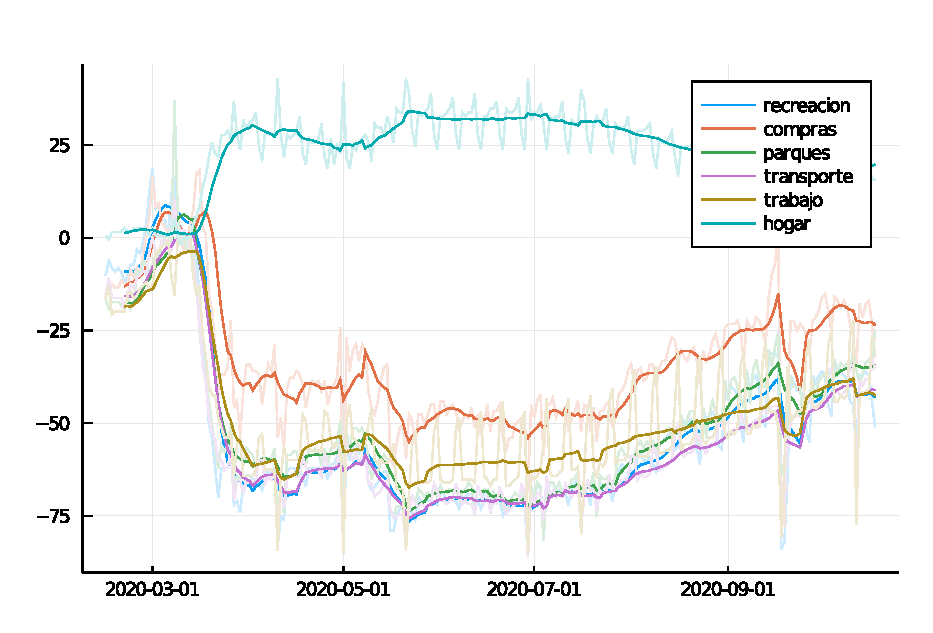
\includegraphics[width=.7\textwidth]{img/metodologia/datos/explorar_movilidad_google_6_1.eps}
\caption{Variación en la movilidad agregada por actividad en la Región Metropolitana y media móvil de 7 días. Fuente: Elaboración propia con datos de Google.}
\label{img:google-movilidad-RM}
\end{figure}


%\noindent \textbf{Uso de infraestructura de telecomunicaciones}
\subsection{Uso de infraestructura de telecomunicaciones}\label{data:isci}

% Acerca de los proveedores
El Instituto Sistemas Complejos de Ingeniería (ISCI), que agrupa a un conjunto de investigadores de varias universidades de Chile con el objeto de generar trabajo científico y desarrollar soluciones para problemas complejos de ingeniería,
% Sus investigadores desarrollan proyectos en las áreas de la Gestión de Operaciones, Ingeniería de Transporte, Optimización y Energía, y otras como Organización Industrial y Medioambiente. Estas áreas comparten herramientas analíticas básicas y se complementan disciplinariamente. 
%[Link ing ISCI, http://ingenieria.uchile.cl/investigacion/centros-y-programas/88242/instituto-sistemas-complejos-de-ingenieria]
 en conjunto con Entel Ocean, la Unidad Digital de Entel, 
compañía de tecnología y telecomunicaciones, recopilaron información acerca del uso de infraestructura de telecomunicaciones.
%Entel:  https://informacioncorporativa.entel.cl/nuestra-compania

% Acerca de la metodologia 
Los datos se encuentran agrupados a nivel de zona censal. La información disponible les permitió deducir la zona hogar, en donde las personas se encuentran frecuentemente en horarios no laborales. Para cada día laboral (lunes a viernes), determinaron el flujo desde cada zona hogar a otras zonas, durante horarios de trabajo. Estos flujos pueden ser dentro de la misma comuna o a otras comunas, y fueron considerados un proxy de la movilidad en Santiago. % Luego, tomaron promedios semanales a nivel de comuna (excluyendo fines de semana) de esos flujos 

Las dos primeras semanas de marzo del 2020, antes de la declaración de la fase 2 de pandemia por COVID-19 en Chile, fueron consideradas como semanas ``base'', siendo una aproximación para la movilidad usual de cada zona \cite{Olivares2020}. Los cambios en movilidad por zona con respecto a esa movilidad base fueron reportados para cada semana, y se encuentran disponibles en el repositorio de la Mesa de Datos del Ministerio de Ciencia, Tecnología, Conocimiento e Innovación \cite{MINCIENCIA}. También pueden verse en el Visor Movilidad en \url{https://covidanalytics.isci.cl/movilidad/visor-movilidad/}, como en la figura \ref{img:ISCI-movilidad-RM}.
%Datos en https://github.com/MinCiencia/Datos-COVID19/tree/master/output/producto51 

La versión completa de estos datos, que contiene información tanto del origen como del destino de los transeúntes, fue analizada en \cite{Carranza2020}. La versión pública de estos datos, sin embargo, solo contiene la movilidad de entrada y salida de cada zona censal/comuna; es posible saber cuánta gente sale y entra a una zona censal o comuna pero no hacia dónde va.

\begin{figure}[H]
\centering
\includegraphics[width=\textwidth]{img/metodologia/datos/ISCI-movilidad-RM.png}
\caption{Variación en la movilidad de cinco comunas de la Región Metropolitana. Fuente: ISCI Covid Analytics.}
\label{img:ISCI-movilidad-RM}
\end{figure}




\subsection{Datos-COVID19}\label{sec:datos-minsal}

La Mesa de Datos COVID-19 liderada por el Ministerio de Ciencia, Tecnología, Conocimiento e Innovación busca proveer de información del país durante la pandemia, con el fin de promover el uso de datos para investigación científica, clínica y para soluciones innovadoras. Dispone de datos documentados del Ministerio de Salud (MINSAL) y de otras fuentes \cite{MINCIENCIA}.

% datos disponibles
La información está organizada en distintos \textit{Data Products}. Existen series de tiempo de casos confirmados, hospitalizados, UCI, conectados a ventilación mecánica, fallecidos, cantidad de exámenes PCR realizados, nacimientos y fallecimientos, cuarentenas, etc. Estos datos son utilizados, por ejemplo, en el visualizador del Centro de Modelamiento Matemático disponible en \url{https://covid-19vis.cmm.uchile.cl/geo}. Algunos ejemplos de estos datos son las figuras \ref{img:cmm-fallecidos} y \ref{img:cmm-vacunados}.

\begin{figure}[H]
\centering
\includegraphics[width=0.9\textwidth]{img/metodologia/datos/fallecidos_nacional.png}
\caption{Total de casos fallecidos por COVID-19 acumulados a nivel nacional. Fuente: Centro de Modelamiento Matemático  con Datos-COVID19.}
\label{img:cmm-fallecidos}
\end{figure}

\begin{figure}[H]
\centering
\includegraphics[width=0.9\textwidth]{img/metodologia/datos/CoberturaVacunacionRM.png}
\caption{Porcentaje de cobertura vacunación COVID-19 en la Región Metropolitana. Fuente: Centro de Modelamiento Matemático con Datos-COVID19.}
\label{img:cmm-vacunados}
\end{figure}



% Justificación de la elección de los compartimientos, basada en las características del Covid en la región que estamos estudiando. 
% Modelo multiclase elegido 

\section{Decisiones específicas acerca del modelo} \label{met:decisiones}

% Compartimientos a usar 
% parámetros fijos y variables 

% Todas las decisiones tomadas con respecto a los compartimientos y los parámetros usados van aquí (si se usó uno común para todos, o se ajustaron por separado, etc). 


% describir el modelo que usan en el artículo, como un ejemplo % mencionar las cosas propias del modelo: multiclase, ambientes, tasa de contagio que usa matriz de tiempos de residencia. describir en detalle la tasa de contagio.

% elegir los compartimientos específicos a usar, susceptibles, expuestos, etc. literatura covid

% parametros fijos y variables, literatura covid (ver la parte de kalman, habia algo interesante ahi

% comentar que este modelo permite modelar mascarillas y esas cosas... un avance según pedro 


% Modelos de covid usualmente utilizados (compartimientos, etc)
% Describir este modelo en particular, usando el numero 1. 

% enfoque tasa de contacto vs tiempo de residencia  

% Esto ya lo discutí al inicio 


En esta sección se tomarán decisiones específicas concernientes a la aplicación de la metodología al caso de estudio. Esto permite decidir el modelo específico a utilizar, lo que incluye la elección de compartimientos a utilizar (susceptibles, expuestos, infectados, etc), parámetros, además de las clases y ambientes. Todo esto debe considerar las características del COVID-19 y también los datos disponibles. 

Ya se ha expuesto previamente en \ref{modelo-clases-vs-ambientes} el modelo de dispersión virtual presentado por \cite{Bichara2015}, el cual permite trabajar simultáneamente con clases y ambientes. Ahora se discute las particularidades del modelo a usar en este caso específico. Es necesario definir los compartimientos y parámetros específicos a usar, considerando la enfermedad a modelar, en este caso el COVID-19.
%A continuación se expone el modelo de dispersión virtual con ambientes de \cite{Bichara2015}. Está basado en un modelo de tipo SIS (\textbf{S}usceptibles, \textbf{I}nfectados). 

% acerca de los compartimientos a usar 

Dependiendo del aspecto de interés, distintos compartimentos han sido usados para modelar el COVID-19. Los modelos revisados por la revisión \cite{Xiang2021} utilizan los clásicos Susceptibles, Infectados, Recuperados, en combinación con Expuestos, Hospitalizados y/o Fallecidos. La existencia de casos asintomáticos que portan el virus y pueden contagiarlo pero no presentan síntomas (o presentan síntomas muy leves) es considerado en algunos modelos. Algunos consideran compartimientos En Cuarentena y el desarrollo de vacunas da lugar a modelos con compartimientos de Vacunados.

Como se exponía inicialmente, se buscaba un modelo epidemiológico que considere un riesgo en tres factores: amenaza, exposición y vulnerabilidad. Suponiendo que hay varias clases \(i \in 1 \dots n\) y ambientes \(j \in 1 \dots m\), la idea propuesta de amenaza era de la forma \(\beta_j I_j/N_j\), que incluía la fracción de infectados en un lugar y un factor \(\beta_j\) dependiente de las características del lugar. Se consideraban además valores \(p_{ij}\), que representaban la fracción de tiempo que la clase \(i\) pasaba en el ambiente \(j\), y un factor sanitario \(\alpha_i\) dependiente de la clase \(i\) y relacionado a las medidas de cuidado personal y la susceptibilidad al contagio. Al combinar lo anterior se obtenía la expresión \ref{eq:idea-1}, que da una idea de la tasa de contagios de la clase \(i\) buscada.

\begin{equation}\label{eq:idea-1}
\alpha_i \sum_{j = 1}^m \beta_j p_{ij} \frac{I_j}{N_j}
\end{equation}

Para hacer de esta idea algo concreto, se vuelve al apartado \ref{modelo-clases-vs-ambientes}, donde se habló del modelo de clases y ambientes propuesto por \cite{Bichara2015}\cite{Bichara2018}. Como antess, se separa a la población en \(n\) clases, las cuales interactúan en \(m\) ambientes o áreas de riesgo. \(N_i(t), i = 1, \dots, n\) corresponde a la población de la clase \(i\). Se supone que la población de la clase \(i\) pasa una proporción \(p_{ij} \in [0,1]\) de su tiempo en el ambiente \(j\), con \(\sum_{j = 1}^{m} p_{ij} = 1\) para cada \(i\). Para casos extremos, por ejemplo, podría darse que \(p_{ij} = 0\), es decir, la clase \(i\) no gasta nada de su tiempo en el ambiente \(j\), mientras que \(p_{ij} = 1\) significa que la clase \(i\) pasa todo su tiempo en el ambiente \(j\). La matriz \(P = \{p_{ij}\}_{i = 1\dots n,j \dots m}\) es llamada matriz de tiempos de residencia. Esta matriz será estimada a partir de los datos disponibles. Más aún, se busca una matriz que sea variable en tiempo, de tal forma que refleje los cambios en el comportamiento de la población a lo largo de la pandemia.


Se decide trabajar con el ampliamente utilizado modelo SEIR; ya ha sido utilizado para estudiar el impacto de las cuarentenas y reducciones de movilidad y viajes \cite{Lai2020}\cite{Chinazzi2020}, demás del uso de mascarillas \cite{Kai2020}, por lo que parece una elección razonable. Las ecuaciones del modelo elegido son \ref{eq:modelo-final}. Se decidió despreciar los efectos demográficos de los nacimientos y fallecimientos naturales de la población. Eso se traduce en tasas de natalidad y mortalidad \(b_i, d_i\) iguales a 0. Esto debido a que no se trabajará a largo plazo, solo con un intervalo de tiempo de poco más de un año.

La matriz de tiempos de residencia \(P(t) = \{p_{ij}(t)\}_{i,j}\) será una variable en el tiempo, la forma de estimarla se expondrá en la sección \ref{met:matriz}. Esto se hará de antemano, antes de correr el modelo, por lo que se considera conocida. Se usará la información conocida acerca del COVID-19 para los valores \(\gamma_{Ei}, \gamma_{Ii}\) y los riesgos específicos de cada ambiente \(\beta_j\) se elegirán antes usando valores plausibles. La estimación del factor sanitario \(\alpha_i(t)\) se presentará en \ref{met:estimacion}.

\begin{equation}\label{eq:modelo-final}
\begin{aligned}
%S_i(t)' &= -S_i(t) {\color{Red} \lambda_i(\vec{x}, t) } \\
S_i'(t) &= - \lambda_i(\vec{x}, t)\\
E_i'(t) &= \lambda_i(\vec{x}, t) S_i(t)  - \gamma_{Ei} E_i(t) \\ 
I_i'(t) &= \gamma_{Ei} E_i(t)  - \gamma_{Ii} I_i(t) \\ 
R_i'(t) &= \gamma_{Ii} I_i(t) \\
\lambda_i(\vec{x}, t) &= \alpha_i(t)\sum_{j=1}^m \beta_{j}p_{ij}(t) S_i(t) \left(\frac{\sum_{k=1}^{n}p_{kj}(t) I_k}{\sum_{k=1}^{n}p_{kj}(t)N_k}\right)
\end{aligned}
\end{equation}

Con respecto a los compartimientos elegidos, se decidió no utilizar uno de Fallecidos. Ahora bien, \cite{Mena2021} menciona que al trabajar con niveles socioeconómicos, la cantidad de fallecidos es muchos más confiable que la de casos infectados detectados debido a problemas de trazabilidad en las comunas de menores recursos, especialmente al inicio de la pandemia. El problema es que la tasa de fallecimiento o la fracción de infectados que fallecen es probablemente variable en tiempo, dependiente de las distintas políticas usadas para enfrentar la pandemia. Se decidió mantener la simplicidad del modelo estimando únicamente el factor sanitario. Por motivos similares, la vacunación no fue considerada, sin embargo, se espera que sus efectos se reflejen directamente en el factor sanitario, al hacer a los vacunados menos vulnerables a una posible infección.


% Hay un estudio que calcula Impact of universal masking. 




% Cada ambiente \(j\) tendrá asociado un riesgo \(\beta_j\). Se impone que el riesgo en el ambiente \texttt{hogar} es \(\beta_{\text{hogar}} = 1\). Todos los demás riesgos deben fijarse relativos a ese valor. Se decide incorporar un factor sanitario \(\alpha_i\), dependiente de la clase, el que se interpreta como un indicador del nivel de respeto por las medidas sanitarias (lavado de manos, uso de mascarillas, guardar la distancia, etc) de la clase \(i\)-ésima. Se supone que los efectos de la movilidad están completamente incluídos en la matriz de tiempos de residencia, por lo que este factor solo considera medidas de cuidado. Se supone además que es variable en el tiempo. 


% \[
% \lambda_i(\vec{x}, P) = \alpha \sum_{j=1}^m \beta_{j}p^S_{ij}
% \left(
% p_E \frac{\sum_{k=1}^{n} r^E_{kj}E_k}{\sum_{k=1}^{n}r^E_{kj}N_k} +
% p_{I} \frac{\sum_{k=1}^{n} r^I_{ kj}I_k }{\sum_{k=1}^{n}r^I_{kj}N_k} +
% p_{I^m} \frac{\sum_{k=1}^{n}r^{I^m}_{kj}I^m_k}{\sum_{k=1}^{n}r^{I^m}_{kj}N_k}
% \right)
% \]



% Otras decisiones ... tal vez en otro lugar 
% UNa vez que se deciden las clases y ambientes. 


% Veamos a qué corresponde cada una de las variables. Considero
% $V \in \{S,E,I,I^m\}$.

% \begin{itemize}
% \itemsep1pt\parskip0pt\parsep0pt
% \item
%   $\beta_j$ es una medida de riesgo por unidad de tiempo del ambiente
%   $j$. Yo diría que corresponde a cantidad de contagiados por día en el
%   ambiente $j$, pero no estoy segura. De ser así, se mediría en
%   personas/día.
% \item
%   $p_{ij}^V \in [0,1]$ corresponde a la fracción de tiempo que gastan
%   las personas en el estado $V$ la clase $i$ en el ambiente $j$. Se mide
%   en días.
% \item
%   $p_{kj}^VV_k$ se mide en días $\cdot$ persona. Su valor máximo es
%   cuando $p_{kj}^V = 1$, ahí vale $V_k$ días $\cdot$ persona (son como
%   las horas $\cdot$ hombre, que en economía es una medida de
%   ``esfuerzo'' necesario para llevar a cabo una actividad). Corresponde
%   al tiempo total invertido por todas las personas de la clase $k$ que
%   están en el estado $V$de la enfermedad en el ambiente $j$. Es el
%   ``trabajo de contagio'' del grupo $V_k$.
% \item
%   Es interesante además considerar $p_{kj}^V N_k$, porque no coincide el
%   estado de la matriz $P$ con el que estamos multiplicando. El el
%   ``trabajo de contagio'' que se realizaría si todas las personas de la
%   clase $k$ se movieran como si estuvieran en el estado $V$. El
%   ``trabajo de contagio'' hipotético que realizaría la clase $k$ si
%   estuvieran todos en estado $V$.
% \item
%   Cuando sumamos en todas las clases $k = 1, \dots, n$ obtenemos
%   $\sum_{k=1}^{n}p^{V}_{kj}V_k$, el ``trabajo de contagio'' del estado
%   $V$ realizado en el ambiente $j$.
% \item
%   La suma del denominador $\sum_{k=1}^{n}p^{V}_{kj}N_k$ corresponde al
%   ``trabajo de contagio'' hipotético que se haría en el ambiente $j$ si
%   toda la población estuviera en el estado $V$.
% \item
%   Visto así, creo que el término $\alpha_V$ es una medida de la
%   efectividad del ``trabajo de contagio''. Debería ser un número en
%   $[0,1]$, pero no estoy segura. Aún no tengo clara la unidad de medida.
%   Podría ser como una medida de productividad. La productividad se
%   mide en (cantidad producida)/(horas $\cdot$ hombre). Tiene sentido
%   creo\ldots{} así se anularía después con el término $S_ip_{ij}$, que
%   se mide en (horas $\cdot$ hombre). Lo especial de ese término es que
%   se usa para comparar entre los distintos estados (debería cumplirse
%   $\alpha_I > \alpha_{I^m}> \alpha_{E}$).
% \item
%   Si ahora consideramos la fracción
%   $\frac{\sum_{k=1}^{n}p^{V}_{kj}V_k}{\sum_{k=1}^{n}p^{V}_{kj}N_k}$, lo
%   que tendríamos es una fracción de ``esfuerzo'', sería algo como:
%   ``trabajo real de contagio de $V$ en $j$''/``trabajo ideal de contagio
%   de $V$''. Recalco lo de ``ideal''.
% \item
%   $S_i(t)\lambda_i(\vec{x},P)$ es un flujo, la tasa a la que se pasa del
%   estado $S$ al estado $E$. Se mide en personas/tiempo. No queda otra
%   alternativa entonces de que el término $\beta_j \alpha_V$ se mida en
%   días$^{-2}$. Eso es extraño\ldots{} debería ser un término de
%   aceleración y no de velocidad como pensé al principio. Eso me da la
%   idea de calcular $S''_i(t)$\ldots{} pero no me llevó muy lejos.
% \item
%   Necesito setear algún valor. Digamos que $\alpha_I = 1$. Luego,
%   $\beta_j p_{ij} \alpha_{I} \frac{\sum_{k=1}^{n} p^I_{ kj}I_k }{\sum_{k=1}^{n}p^I_{kj}N_k}$
% \item
%   Necesito llevar esa cantidad a contagios/tiempo. Necesito una medida
%   de la eficiencia del trabajo de contagio. Eso debería medirse en
%   contagios/(hora $\cdot$ persona).
% \end{itemize}


% Elección de matriz de tiempos de residencia 
% Cómo variarla en el tiempo (sección por trabajar)
% Justificación de la elección de ambientes, basada en los que hayan sido importantes, los que aparecen en los datos, etc. 
\section{Matriz de tiempos de residencia}\label{met:matriz}

En la sección anterior se planteó el modelo multiclase multiambiente a utilizar. La principal diferencia con respecto a otros modelos multiclase está en la forma en que se calculaba la tasa de contagio; las \(n\) clases interactúan en \(m\) ambientes virtuales. Esta interacción está codificada por medio de la matriz de tiempos de residencia \( P =\{p_{i,j}\}_{i \in 1 \dots n, j \in 1 \dots m}\), donde la entrada \(p_{ij}\) corresponde a la fracción del día que la clase \(i\) pasa en el ambiente \(j\).

El objetivo de este apartado es elegir las clases y ambientes a utilizar para estudiar el caso de Santiago, y estimar la matriz \(P\) de tiempos de residencia asociada. Es importante notar que se desea que esta matriz sea variable en el tiempo, puesto que las diferentes medidas de mitigación como cierre de instituciones educativas, cuarentenas, etc. implementadas por el gobierno de Chile han cambiado significativamente el modo de vida en la ciudad.  

Se comienza eligiendo las clases y ambientes a utilizar, en la subsección \ref{subsec:eleccion-clases-ambientes}. Posteriormente, en \ref{subsec:santiago-normal-eod}, se describirá la metodología para la obtención de una matriz de tiempos de residencia \(P^0\) correspondiente a la ciudad de Santiago en condiciones normales. Finalmente, en \ref{subsec:variaciones}, se describirá la metodología para modificar esta matriz, con el fin de reflejar las variaciones en el comportamiento de la población a lo largo del desarrollo de la pandemia, lo que da lugar a la matriz \(P(t)\) definitiva. Esta idea de estimar una matriz de comportamiento normal para luego modificarla ha sido desarrollada también por \cite{Lai2020}.


\subsection{Elección de clases y ambientes}\label{subsec:eleccion-clases-ambientes}

El impacto de la enfermedad ha sido heterogéneo entre la población. Se sabe que la edad es un factor a considerar; la susceptibilidad a la infección y la probabilidad de desarrollar síntomas luego del contagio aumentan con la edad \cite{Davies2020}. Similarmente, tanto el porcentaje de infectados cuya gravedad requiere hospitalización como el porcentaje que termina falleciendo es más alto entre los adultos mayores \cite{Verity2020}. El nivel socioeconómico tampoco puede ser ignorado; el menor acceso a la salud \cite{Wang2020}, sumado al desempleo y la mayor presencia de enfermedades crónicas previas \cite{Ahmed2020} son un agravante que hace más vulnerables a los niveles socioeconómicos más pobres.

Hay varios criterios a considerar a la hora de elegir las clases y los ambientes. En primer lugar, es ampliamente conocido \cite{Davies2020}\cite{Verity2020} que la edad es un factor importante en el efecto de la enfermedad en una persona; el COVID-19 afecta con más intensidad a los adultos mayores. Varios estudios \cite{Wang2020}\cite{Ahmed2020}\cite{Chang2021}\cite{Mena2021}\cite{Bennett2021} han mostrado que la pandemia ha afectado más fuertemente a los niveles socioeconómicos o comunas más pobres y lo asocian, entre otras cosas, a la dificultad de ellos de acatar las cuarentenas, junto con menor trazabilidad y peor acceso a cuidados de la salud. Puesto que la Encuesta Origen Destino muestra diferencias en el uso del tiempo entre hombres y mujeres \cite{Jara-Diaz2013}, el sexo podría ser una variable a considerar también.

Los datos disponibles considerados en \ref{sec:datos-disp} han de ser considerados también. La Encuesta Origen Destino, por un lado, posee datos muy granulares; es posible conocer para cada individuo su sexo, zona censal y comuna donde reside, edad e ingreso familiar. Más aún, los distintos propósitos de los viajes realizados (regreso al hogar, al trabajo, escuela, compras, transporte público, bicicleta, entre otros) entregan varios ambientes donde ese individuo pasa su tiempo. 

Por otro lado, las demás fuentes de datos no poseen tanta información. El Uso de infraestructura de telecomunicaciones permite conocer cómo ha cambiado la movilidad de entrada o salida a cada zona censal/comuna, pero no distingue entre las actividades que realizan las personas mientras se mueven por la ciudad. Los Informes de Movilidad Local sobre COVID-19 de Google permiten distinguir distintas actividades, pero no permiten separar por comuna. Las series de tiempos de Datos-COVID19 presentan dificultades similares. Están desagregadas por edad, sexo o comuna, pero no por los tres criterios simultáneamente. 

Puesto que se desea considerar el efecto de las cuarentenas en el uso del tiempo de las personas a lo largo de la pandemia, sabiendo la importancia que juega en las diferencias entre las distintas comunas, se decide usar los datos de movilidad vistos en la sección \ref{data:isci}. Se decide desechar la información de los distintos ambientes; solo se sabe que hay más o menos movilidad fuera del hogar, pero no se sabe exactamente en qué actividad. El trabajo realizado considera, por tanto, solo \(m = 2\) ambientes: \texttt{hogar} y \texttt{exterior}. Es interesante mencionar que el modelo del \textit{Imperial College} \cite{Ferguson2020} considera que del total de contagios, aproximadamente 1/3 ocurren en el hogar, 1/3 en el trabajo y/o entidades educativas, y el último 1/3 en otras actividades como compras o recreación, en concordancia con matrices de mezcla social como \cite{Mossong2008}.

Los datos elegidos permiten utilizar la información a nivel de zona censal, pero los datos epidemiológicos no son tan granulares, por lo que es más factible distinguir por comuna. Los datos epidemiológicos están disponibles a este nivel también, por lo que es una buena posibilidad. Eso, sin embargo, plantearía un sistema con unas 50 clases, lo que para 4 compartimientos da unas 200 variables; es posible, aunque agrega más carga computacional y dificulta el análisis posterior. Se decide, por simplicidad, reducir el análisis a \(n = 5\) categorías socioeconómicas, las mismas propuestas por \cite{SEREMIRM2019}, que surgen tras ordenar las comunas por IPS, como describe la sección \ref{sec:ips}. La tabla \ref{table:ips-categ} muestra un resumen de las categorías elegidas, la versión completa se encuentra en la tabla \ref{table:ipsfull}. 

% Agregar población según CENSO 
\begin{table}[h!]
\centering
\begin{tabular}{||c | c | c | c||} 
 \hline
 \textbf{Prioridad Social} & \textbf{IPS mínimo} & \textbf{IPS máximo} & \textbf{Ejemplos} \\ [0.5ex] 
 \hline
 Alta & 78.24 & 83.03 & La Pintana, Lo Espejo\\ 
 Media Alta & 73.84 & 77.39 & San Bernardo, El Bosque\\
 Media Baja & 65.05 & 71.36 & La Cisterna, Quinta Normal\\
 Baja & 53.34 & 64.37 & Santiago, Providencia\\
 Sin Prioridad & 6.26 & 37.36 & Las Condes, Lo Barnechea\\ [1ex] 
 \hline
\end{tabular}
\caption{Resumen de las categorías socioeconómicas por IPS, dadas por \cite{SEREMIRM2019}.}
\label{table:ips-categ}
\end{table}



\subsection{Matriz de Santiago en condiciones normales} \label{subsec:santiago-normal-eod}

% Acerca de los propósitos de viajes 
% Los propósitos son los siguientes:
% Al trabajo
% Por trabajo
% Al estudio
% Por estudio
% De salud
% Visitar a alguien
% Volver a casa
% Buscar o Dejar a alguien
% Comer o Tomar algo
% Buscar o dejar algo
% De compras
% Trámites
% Recreación
% Otra actividad 
En \cite{Munizaga2011} se propone un método para obtener información acerca del uso del tiempo de una persona a partir de los tiempos de inicio y fin de sus viajes y el propósito declarado de este, datos contenidos en la Encuesta Origen-Destino. Para esto supone que el primer viaje comienza desde el hogar y luego cada período de tiempo entre dos viajes consecutivos es asignado a la actividad declarada como propósito en el viaje anterior. La Figura \ref{img:ciclo-viajes} es un diagrama de este proceso. 
% Insertar el algoritmo para esto, traducir 

\begin{algorithm}[H]
\SetAlgoLined

\KwIn{
Una lista de personas \(P\). Para cada \(p \in P\), una lista \(V_p\) de todos los viajes hechos por \(p\), ordenados del primero al último. Para un viaje \(v\) es posible obtener \(t_0, t_f\) tiempos de inicio y fin, \(\mathtt{modo}\) de transporte y \(\mathtt{prop\acute{o}sito}\) del viaje.
Dos funciones \( \mathcal{J}_{\mathtt{m}}: \mathtt{modo} \mapsto j\) y \(\mathcal{J}_{\mathtt{p}}: \mathtt{prop\acute{o}sito} \mapsto j\) que asocian cada \texttt{modo} de transporte (bus, auto, etc) y cada \texttt{propósito} de viaje (al trabajo, de compras, etc) a un ambiente \(j \in \{1, \dots, m\}\) (trabajo, compras, transporte público, etc). Un ambiente por defecto \(j_0\) (hogar), donde las personas sin viajes pasan su tiempo, y donde las personas comienzan su primer viaje. Una función \(\mathcal{C}: p \in P \mapsto i\) que asigne a cada persona \(p\) una clase \(i \in \{1, \dots, n\}\). Tiempos de inicio \(T_0\) y fin \(T_f\) del intervalo de tiempo total considerado.
}

\KwResult{Una matriz de tiempos de residencia \(R = (r_{ij})_{i = 1 \dots n, j = 1 \dots m}\) donde \(r_{ij}\) es la fracción del tiempo que la clase \(i\) pasa en el ambiente \(j\). Solo considera personas sin viajes inválidos.}

%Elegir un grafo $G$ conexo y una matriz $R$. 

Definir la matriz auxiliar \(C = (c_{ij})_{i = 1 \dots n, j = 1 \dots m}\). \(c_{ij}\) guardará el tiempo total que las personas de la clase \(i\) pasan en el ambiente \(j\). Se inicializa en \(0\)\;

Definir \(T = T_f - T_0\) el tiempo total considerado.

Definir \(N_i \gets 0\) para cada \({i \in 1 \dots n}\) para contar el total de personas en cada clase. 

\ForAll{\(p \in P\)}{
    Guardar en \(i\) el valor \(\mathcal{C}(p)\), la clase de \(p\)\; %\tcc*[r]{class of person \(p\)} \;

    \uIf{La persona \(p\) no tiene viajes, \(V_p = \varnothing\)}{
        Se supone que \(p\) pasa todo su tiempo en el ambiente \(j_0\) por defecto. \(c_{i,j_0} \gets c_{i,j_0} + T\)\; 
        
        Contabilizar una persona válida. \(N_i \gets N_i + 1\)\;
    }
    \uElseIf{\(V_p\) tiene información faltante (\(\mathtt{prop\acute{o}sito}, \mathtt{modo}, t_0\) or \(t_f\) de algún \(v \in V_p\) no está definido)}{
        \(p\) no es una persona válida y no es considerada en la matriz final\;
    }
    \Else{
        \(j\_\mathtt{anterior} \gets j_0 \). Ambiente donde terminó el viaje anterior. Comienza en \(j_0\)\;
        \(t_f\_\mathtt{anterior} \gets T_0\). Hora de término del viaje anterior. Vale \(T_0\) por defecto\;
        \ForAll{viaje \(v \in V_p\)}{
            Obtener \(\mathtt{prop\acute{o}sito}, \mathtt{modo}, t_0\) y \(t_f\) asociados al viaje \(v\). Definir \(j_v \gets \mathcal{J}_\mathtt{m}(\mathtt{modo})\) el ambiente asociado al modo del viaje \(v\)\;
            
            Agregar el tiempo entre el viaje anterior y el viaje \(v\) al ambiente donde terminó el viaje anterior. \(c_{i, j\_\mathtt{anterior}} \gets c_{i, j\_\mathtt{anterior}} + t_s - t_f\_\mathtt{anterior}\)\;
            
            Agregar el tiempo del viaje \(v\) a su ambiente asociado. \(c_{i, j_v} \gets c_{i, j_v} + t_f - t_s\)\;
            
            Actualizar  \(j\_\mathtt{anterior} \gets \mathcal{J}_{\mathtt{p}}(\mathtt{prop\acute{o}sito})\). El próximo viaje comienza donde \(v\) terminó.
            
            Actualizar \(t_f\_\mathtt{anterior} \gets t_f\). 
        }
        
        Agregar el tiempo entre el último viaje y el tiempo final \(T_f\) \(v\) al ambiente donde terminó el último viaje. \(c_{i, j\_\mathtt{anterior}} \gets c_{i, j\_\mathtt{anterior}} + T_f - t_f\_\mathtt{anterior}\)\;
        
        Contabilizar a \(p\) como una persona válida. \(N_i \gets N_i + 1\)\;
    }
    
}

Calcular \(R\) a partir de \(C\) normalizando cada fila. \(r_{ij} \gets c_{ij} / T N_i\)\;

\caption{Tiempos de residencia a partir de una lista de viajes}
\label{alg:timematrix}
\end{algorithm}

\begin{figure}[H]
\centering
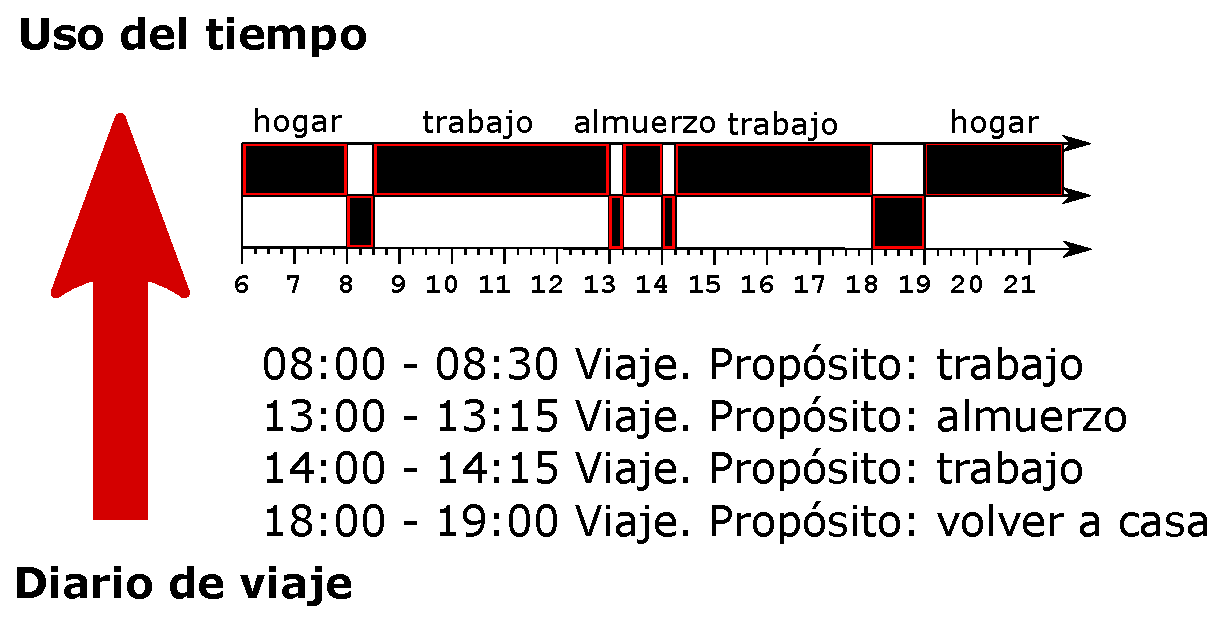
\includegraphics[width=.6\linewidth]{img/metodologia/matrizPnormal/ciclo-viajes.eps}
\caption[Transformar propósitos de viaje en tiempo de actividad.]{Transformar propósitos de viaje en tiempo de actividad. Fuente: \cite{Munizaga2011}, traducción propia.}
\label{img:ciclo-viajes}
\end{figure}

El algoritmo \ref{alg:timematrix} explica el proceso en detalle de manera general. Cabe mencionar que este algoritmo fue desarrollado de manera independiente y con importantes variantes antes de conocer \cite{Munizaga2011}. Este algoritmo es aplicado para construir una matriz detallada de tiempos de residencia, intentando aprovechar la mayor información posible de los propósitos de viajes. También es usado para construir la matriz de tiempos de residencia con únicamente dos ambientes, pero en ese caso las funciones \(\mathcal{J}_{\mathtt{p}}\), \(\mathcal{J}_{\mathtt{m}}\) son considerablemente más sencillas; solo el propósito asociado con ir al hogar se asocia al ambiente \texttt{hogar} y todos los demás se asocian a \texttt{exterior}. La matriz obtenida usando este algoritmo se denota \(P^0\). La matriz variable en el tiempo será construida a partir de esta en la siguiente subsección. 
% Creo que sería bueno agregar el pseudo código de la cuestión. Estoy segura de que yo tenía una versión bonita de esto.
% Para que sea replicable tengo que incluir todas las pequeñas decisiones... los casos usados y los no usados, todo eso. 

% Proceso de manera diferenciada a los no viajeros de los viajeros. Se asume que los primeros pasan todo su tiempo en el hogar. 

% Redirigir a la imeplementación en Matlab.


\subsection{Variaciones de la matriz a lo largo del tiempo} \label{subsec:variaciones}

% Explicar los datos disponibles
Se usan los datos de movilidad obtenidos del Uso de infraestructura de telecomunicaciones, descritos en \ref{data:isci}. Los datos se obtienen del repositorio de Datos-COVID19, descrito en \ref{sec:datos-minsal}, del Producto 82 específicamente. 
% Nos estoy segura de qué tanto detalle tengo que dar aquí, puedo ser muy específica y describir hasta las columnas involucradas. Tal vez como un anexo... 

% Los datos se encuentran en dos archivos en formato \texttt{.csv}, correspondientes a la movilidad durante días laborables de la semana \texttt{ISCI\_weeks.csv} y a la movilidad de los fines de semana \texttt{ISCI\_weekends.csv}. Se usa solo el primero de estos. Los atributos incluyen la comuna de la Región Metropolitana con nombre, \texttt{nom\_comuna} y código único territorial \texttt{comuna} a la que corresponde la medición, semana epidemiológica \texttt{semana} de la medición con fecha de inicio \texttt{fecha\_inicio} y fin \texttt{fecha\_termino}, y estimaciones de la variación de movilidad \texttt{var\_salidas}, que es un promedio entre \texttt{var\_salidas\_cota\_superior} y \texttt{var\_salidas\_cota\_inferior}. 

Los datos se encuentran en dos archivos en formato \texttt{.csv}, correspondientes a la movilidad durante días laborables de la semana y a la movilidad de los fines de semana. Se usa solo el primero de estos. Los atributos incluyen la comuna de la Región Metropolitana con nombre y código único territorial, comuna a la que corresponde la medición, semana epidemiológica de la medición con fecha de inicio y fin, y estimaciones de la variación de movilidad, con cotas inferiores y superiores.

Se utiliza la información de estimaciones de la variación de movilidad (despreciando las cotas inferiores y superiores). Si llamamos \(m_i^0\) a la movilidad de referencia inicial para la comuna \(i\)-ésima (la cual es desconocida), y \(m_i^k\) a la movilidad de la comuna \(i\)-ésima en la semana \(k\)-ésima posterior a esa semana de referencia, entonces son reportados los valores \(p_i^k\) que satisfacen la ecuación \ref{eq:mov-1}.

\begin{equation}\label{eq:mov-1}
m_i^k = p_i^k m_i^0.
\end{equation}

Un detalle a considerar es que es necesario calcular la variación de movilidad para los distintos grupos socioeconómicos, puesto que solo se tiene para las comunas. Si la población de la comuna \(i\)-ésima es \(N_i\), e \(I\) es un conjunto de comunas, se estima la movilidad grupal con las ecuaciones \ref{eq:mov-2}. Se busca un parámetro \(p_I^k\) tal que \ref{eq:mov-3}. Bajo el supuesto \(m_i^0 := m^0\) para cada \(i\), entonces es fácil ver que se cumple \ref{eq:mov-4}.

\begin{equation}\label{eq:mov-2}
m^k_I = \sum_{i \in I}m^k_i N_i,
\end{equation}


\begin{equation}\label{eq:mov-3}
m_I^k = p_I^k m_I^0,
\end{equation}


\begin{equation}\label{eq:mov-4}
p_I^k = \sum_{i \in I} p_i^k N_i.
\end{equation}

Se supondrá que la movilidad es constante a lo largo de la semana, incluyendo fines de semana, aunque no se considerarán estos datos. Se define una función \(\mathtt{semana}(t)\) que a un tiempo \(t\) le asocia la correspondiente semana. Suponemos además que el tiempo que cada clase pasa en el ambiente \texttt{exterior} varió de manera proporcional a la movilidad. Eso permite calcular la columna \texttt{exterior} de la matriz de tiempos de residencia para cada grupo socioeconómico \(I\) con las ecuaciones \ref{eq:mov-5}. Finalmente, el tiempo que no se ocupa en el ambiente \texttt{exterior} se pasa en el ambiente \texttt{hogar}, por lo que se cumple \ref{eq:mov-6}.

\begin{equation}\label{eq:mov-5}
r_{I, \text{exterior}}(t) = p_I^{\mathtt{semana}(t)} r_{I,\text{exterior}}^0,
\end{equation}

%% Definir una variable para el nombre del ambiente fuera del hogar o exterior 



% Finalmente la matriz de tiempos de residencia que varía en el tiempo 


\begin{equation}\label{eq:mov-6}
r_{I, \text{hogar}}(t) = 1 - r_{I,\text{exterior}}(t).
\end{equation}

% Estimación de parámetros 
\section{Estimación de parámetros} \label{met:estimacion}

% Criterios a considerar... algunos deben ser constantes y otros variables. 

\subsection{Filtro de Kalman}


%Por qué filtro?
Para hacer estimación de parámetros \textit{online} hay varias opciones disponibles; Filtro de Mínimos Cuadrados Recursivo (\textit{Recursive Least Squares}) y su extensión el Filtro de Kalman, permiten estimar un estado a partir de su dinámica  y mediciones de alguna variable. Hay alternativas como el filtro de partículas, más costoso computacionalmente, o el filtro por ensambles. Cada uno tiene su propias deficiencias [referencias]. 

% por qué kalman? No un filtro de partículas? EnkF por qué no? H_infty?



%Filtro de Kalman para sistemas continuos no lineales
%Hay muchas alternativas, por qué usar el filtro extendido existiendo también UKF o CKF? No se necesitaba tanto poder de cómputo tampoco...

Filtro de Kalman fue desarrollado en primera instancia como un método para tratar sistemas lineales discretos [verificar]. No hay una única forma de trabajar con sistemas continuos no lineales; por una parte, es posible discretizar el sistema mediante métodos como Euler o Runge-Kutta, para luego tratar la no linealidad (este método es llamado \textit{discreto-discreto} en \cite{Kulikov2014}. Por otra parte, es posible linealizar el sistema primero, lo que da lugar al filtro \textit{continuo-discreto}.

Tratar con la no linealidad del sistema puede hacerse de varias formas. La más directa es simplemente linealizar, lo que da lugar al Filtro de Kalman Extendido (EKF por sus siglas en inglés). Hay enfoques más sofisticados que funcionan mejor para problemas altamente no lineales como el \textit{Unscented Kalman Filter} (UKF) (Filtro de Kalman ``sin olor'') o el \textit{Cubature Kalman Filter} (CDF) que se basan estimar la media y varianza de una distribución a la que es aplicada una función no lineal, mediante la evaluación de esa función en varios puntos estratégicamente elegidos, llamados \(\sigma\)-puntos \cite{Kulikov2017}\cite{Simon2006}. Por simplicidad de la implementación y a la hora de chequear observabilidad local, se decidió utilizar EKF en su versión discreta-discreta. La misma decisión fue tomada por \cite{Hasan2020}, pero se prefirió utilizar una discretización de Runge-Kutta de orden 4 en lugar del método de Euler progresivo por estabilidad numérica.


%Por qué usar smoother, qué pasa al usar kalman normal, etc, en qué situaciones habría que usaar kalman... (forecasting por ejemplo).

Debido a que se trabajará con datos pasados y no se hará estimación \textit{online} ni predicción, se utiliza suavizado en lugar de filtraje [referencia a 2.2]. El suavizado será de intervalo fijo, como se explica en [2.2.5], y se usará su versión más conocida, el \textit{Rauch, Tung y Striebel Smoother} o \textit{RTS Smoother} \cite{}\cite{Simon2006}. Esto permite obtener mejores estimaciones, pero solo es posible debido a que disponemos de todas las observaciones para un intervalo de tiempo fijo, y que deseamos la mejor estimación posible dadas esas observaciones. Para estimación \textit{online} solo se cuenta con las mediciones hasta el intervalo donde se quiere estimar, no hay observaciones futuras, lo que lleva a usar filtraje.



\subsection{Modelo}

Para fijar ideas, se comienza con un modelo de una sola clase 
\begin{equation}
\begin{aligned}
S'(t) &= -\alpha S(t)\big( p_E E(t) + p_{I^m}I^m(t) + p_I I(t)\big) \\
E'(t) &= \alpha S(t)\big( p_E E(t) + p_{I^m}I^m(t) + p_I I(t)\big) - \gamma_E E(t) \\ 
(I^m)'(t) &= (1-\phi) \gamma_E E(t) - \gamma_{I^m} I^m(t)\\
I'(t) &= \phi \gamma_E E(t) - \gamma_{I} I(t)\\
R'(t) &= \gamma_{I} \big( I^m(t) + I(t) \big)
\end{aligned}
\end{equation}

donde, como de costumbre, \(S\) corresponde a los susceptibles, \(E\) a los expuestos, \(I^m\) a los infectados sintomáticos, \(I\) a los infectados sintomáticos y \(R\) a los recuperados. \(\gamma_E\) corresponde a la tasa de salida de ... medida en \([\text{día}]^{-1}\), de tal forma que \(\gamma_E^{-1}\) es el período de incubación medido en \(\text{día}\)s. \(\gamma_{I^m}\) y \(\gamma_I\) corresponden a las tasas de recuperación de los infectados asintomáticos y sintomáticos respectivamente. \(\phi\) es la fracción de infectados que son sintomáticos. Consideraremos \(\alpha\) como proporcional a la tasa de contagios.

\subsection{Estimación de la tasa de contagios}

Siguiendo la misma línea que \cite{Hasan2020}, \cite{Hasan2021}, \cite{Hasan2021a}, supondremos que \(\gamma_E\) y \(\gamma_I\) son constantes y que \(\alpha(t)\) es variable y depende de las distintas medidas sanitarias implementadas.


Se cuenta con datos de los casos sintomáticos acumulados, que se calculan como 

\[
C_i(t) = \int_{t_0}^t \gamma_E E_i(s) ds
\]

\noindent \textbf{Modelo con una clase}

Para fijar ideas, se trabaja con el modelo SEIR clásico de una sola clase, incorporando ruido:

\begin{equation}
\begin{aligned}
S'(t) &= -\alpha(t) S(t)I(t) + g_1 w_1(t)\\
E'(t) &= \alpha(t) S(t)I(t) - \gamma_E E(t) + g_2 w_2(t)\\
I'(t) &= \gamma_E E(t) - \gamma_{I} I(t) + g_3 w_3(t)\\
R'(t) &= \gamma_{I} I(t) + g_4 w_4(t)\\
\end{aligned}
\end{equation}

\(w_1, \dots, w_4\) son procesos brownianos independientes entre sí, ponderados por constantes \(g_1, \dots, g_4\).
Se supondrá que \(\gamma_E, \gamma_{I^m}\) y \(\gamma_I\) son conocidos, y se busca estimar \(\alpha(t)\) a partir de observaciones ruidosas de los casos infectados acumulados. Se trabajará con un modelo aumentado, agregando las ecuaciones \ref{eq:simple-augmented-eqs} a la dinámica. \ref{eq:simple-c} permite guardar los casos acumulados en un estado, lo que facilita plantear la ecuación de observación. \ref{eq:simple-alpha} agrega \(\alpha\) a la dinámica sin ser modificada por ella, de forma que solo es actualizada por el paso de análisis del filtro de Kalman.

\begin{subequations}\label{eq:simple-augmented-eqs}
\begin{align}
C'(t)       &= \gamma_E E(t) \label{eq:simple-c} \\ 
\alpha'(t)  &= 0    \label{eq:simple-alpha}
\end{align}
\end{subequations}

Llamando \(\mathbf{x} = (S, E, I, R, C, \alpha)^{\top}\), se obtiene la ecuación de estado \ref{eq:simple-estado}, con parámetros conocidos \(p = (\gamma_E, \gamma_I)\). \(\mathbf{G}\) es una matriz diagonal que pondera el ruido, y \(\mathbf{w}\) un vector de brownianos independientes. Si bien \(f_p\) no depende del tiempo de manera explícita, al trabajar con el modelo completo si habrá dependencia, por lo que se decidió escribir \(f_p(\mathbf{x}, t)\) en lugar de simplemente \(f_p(\mathbf{x})\).

\begin{equation} \label{eq:simple-estado}
\mathbf{x}'(t) =
\begin{pmatrix}
S \\
E\\
I\\
R\\
C\\
\alpha 
\end{pmatrix}' = 
\begin{pmatrix} 
-\alpha(t) S(t)I(t) \\
\alpha(t) S(t)I(t) - \gamma_E E(t) \\ 
\gamma_E E(t) - \gamma_{I} I(t)\\
\gamma_{I} I(t) \\
\gamma_E E(t) \\
0
\end{pmatrix} + \mathbf{G} w(t)= f_p(\mathbf{x}, t) + \mathbf{G} \mathbf{w}(t)
\end{equation}

Para utilizar el filtro discreto-discreto, se requiere discretizar la dinámica \(f_p\), para lo que se usa un esquema de Runge Kutta de orden 4. Para un instante de tiempo \(t_k\), un intervalo de tiempo \(\Delta t\) y un estado \(\mathbf{x}_k\), y definiendo \(\mathbf{x}_1, \dots, \mathbf{x}_4\) como en \ref{}, \ref{eq:simple-rk4} permite obtener una estimación \ref{eq:simple-estado-discreto} para \(\mathbf{x}_{k+1}\). Esto corresponde a la ecuación de estado discretizada, la cual es no lineal.

\begin{equation} \label{eq:simple-rk4}
\mathbf{x}_{k} + \frac{1}{6}\Big( \Delta \mathbf{x}_1  +  2\Delta \mathbf{x}_2 + 2\Delta \mathbf{x}_3 +\Delta \mathbf{x}_4\Big) =: \mathcal{F}_{p, \Delta t}(\mathbf{x}_k, t_k)
\end{equation}


\begin{equation} \label{eq:simple-estado-discreto}
\mathbf{x}_{k+1} = \mathcal{F}_{p, \Delta t}(\mathbf{x}_k, t_k) +  \mathbf{G}\mathbf{w}_{k} 
\end{equation}

Notamos que \(\mathbf{w}_{k} \sim \mathcal{N}(\mathbf{0}, \mathbf{Q}_k)\) y \(\mathbf{Q}_k = \Delta t \text{\textbf{Id}}\) [explicación].

Ahora es necesario trabajar con la no linealidad, lo que se hará mediante el Filtro de Kalman Extendido, expuesto en la sección \ref{filtro-extendido}. Para eso, es necesario calcular el jacobiano de la función \(\mathcal{F}_{p, \Delta t}\). Múltiples usos de la regla de la cadena más la definición del esquema de RK4 dada por \ref{eq:rk4} permiten obtener las ecuaciones \ref{eq:simple-jacobian}.

\begin{equation}\label{eq:simple-jacobian}
\begin{aligned}
D_x(\mathcal{F}_{p, \Delta t})(x_k, t_k) &= I + \frac{1}{6}\Big( D_x h_1  +  2 D_x h_2 + 2D_x h_3 +D_x h_4\Big) \\
t_{k + 1/2} &:= t_k + \Delta t / 2\\
h_1 &= f(x_k, t_k) \\
D_x h_1 &= D_x f(x_k, t_k)\\
h_2 &= \Delta t f(x_k + h_1, t_{k + 1/2}) \\
D_x h_2 &= \Delta t D_x f(x_k + h_1, t_k) (I + D_x h_1)  \\
h_3 &= \Delta t f(x_k + h_2, t_{k + 1/2}) \\
D_x h_3 &= \Delta t D_x f(x_k + h_2, t)(I + D_x h_2) \\
h_4 &= \Delta t f(x_k + h_3, t_{k + 1}) \\
D_x h_4 &= \Delta t D_x f(x_k + h_3, t)(I + D_x h_3) \\
\end{aligned}
\end{equation}

%%%%%%%%%%%%%%%%%%%%%%%%%%%%%%%%%%%%%%
% Observación 
%%%%%%%%%%%%%%%%%%%%%%%%%%%%%%%%%%%%%%

La ecuación de observación \ref{eq:simple-obs} consiste, en primera instancia, simplemente en una matriz que obtiene la coordenada de los casos acumulados \(C\) dentro del vector \(\mathbf{x}\). La observación se obtiene con ruido, dado por \(\mathbf{v}_{k} \sim \mathcal{N}(\mathbf{0}, \mathbf{R}_k)\). 


\begin{equation} \label{eq:simple-obs}
\mathbf{y}_{k} = 
\begin{bmatrix}0 & 0 & 0 & 0 & 1 & 0\end{bmatrix} \mathbf{x}_{k} + \mathbf{v}_k
\end{equation}

Debe mencionarse que el sistema no lineal tiene restricciones; por una parte, al elegir \(b_i = d_i = 0\) se impone que el total de la población debe mantenerse constante. Por otra parte, las variables de estado deben ser positivas para que tengan sentido. El survey \cite{Simon2010} presenta varias alternativas para tratar con restricciones, y se decide usar la técnica de \textbf{Observaciones (casi) perfectas} para mantener constante el total de la población. Para la positividad de las variables, se decide simplemente aplicar la función \(\max(0, x)\) al estado después de los pasos de \textit{forecasting} y análisis.

La idea de Observaciones (casi) perfectas es la siguiente: en un sistema de la forma \(x_{k+1} = f_k(x_k) + w_k\), observado mediante una ecuación \(y_k = Hx_k + v_k \), se busca imponer una restricción \(|Dx - d| \leq \epsilon\). Esto se consigue ampliando la matriz de observaciones como muestra la ecuación \ref{eq:perfect-obs}. Si se busca una restricción fuerte con \(\epsilon = 0\), la técnica es llamada Observaciones perfectas, y si se busca una restricción suave con \(\epsilon > 0\), recibe el nombre de observaciones casi perfectas.


\begin{equation}\label{eq:perfect-obs}
\begin{bmatrix}
y_k \\
d 
\end{bmatrix} = 
\begin{bmatrix}
H \\
D
\end{bmatrix} x_k
+
\begin{bmatrix}
v_k \\
\epsilon  
\end{bmatrix}
\end{equation}

Se elige usar una restricción suave para imponer \(S(t) + E(t) + I(t) + R(t) \approx N\), con lo que se obtiene la ecuación de observación \ref{eq:simple-obs-perfect} definitiva.

\begin{equation} \label{eq:simple-obs-perfect}
\begin{bmatrix}
\mathbf{y}_{k} \\
N
\end{bmatrix} = 
\begin{bmatrix}
0 & 0 & 0 & 0 & 1 & 0 \\
1 & 1 & 1 & 1 & 0 & 0 \\
\end{bmatrix}
\mathbf{x}_{k} + 
\begin{bmatrix}
\mathbf{v}_k \\
\epsilon
\end{bmatrix} =
\begin{bmatrix}
C_k \\
S_k + E_k + I_k + R_k
\end{bmatrix}
 + 
\begin{bmatrix}
\mathbf{v}_k \\
\epsilon
\end{bmatrix}
\end{equation}
Finalmente, a modo de resumen; se utiliza el Filtro de Kalman Extendido sobre el sistema dado por \ref{eq:simple-estado-discreto}. Este sistema fue obtenido extendiendo un modelo SEIR con la variable \(C\) de casos acumulados, y con un factor \(\alpha\) de la tasa de contagio, y discretizado mediante el esquema RK4. El sistema es no lineal en el estado, y lineal en el ruido. La linearización se obtiene a partir del jacobiano calculado en \ref{eq:simple-jacobian}. Para asegurar la positividad de las variables se aplica la función \(\max(x, 0)\) después de cada paso de \textit{forecast} y análisis. Para imponer que la población se mantenga constante, se usa la técnica de observaciones casi perfectas de \cite{Simon2010}. La ecuación de observación final es \ref{eq:simple-obs-perfect}, la cual es lineal.

Una vez calculadas las iteraciones de filtro de kalman, es posible obtener los resultados suavizados con el \textit{RTS smoother} mencionado en la sección \ref{smoother}. Los detalles de la implementación se encuentran en \ref{}.\\



\noindent \textbf{Modelo multiclase}

Al trabajar con el modelo con una clase ya se ha tratado la mayor parte del problema. Ahora se extiende esa metodología al modelo con \(n\) clases y \(m\) ambientes presentado en \ref{met:decisiones}. Se define el vector de variables de estado \(\mathbf{x} = (S_1, \dots, S_n, E_1, \dots, E_n, I_1, \dots, I_n, R_1, \dots, R_n)\). Se supone que \(\gamma_E, \gamma_I, \beta_1, \dots, \beta_m\) son conocidos y fijos, y que son los mismos para cada clase. Las ecuaciones para \(i \in 1\dots n\) están en \ref{eq:full-model}.


\begin{subequations}\label{eq:full-model}
\begin{align}
S_i'(t) &= -\lambda_i(\mathbf{x}, t) S_i(t) + g^S_i w^S_i(t)\\
E_i'(t) &= \lambda_i(\mathbf{x}, t) S_i(t) - \gamma_E E_i(t) + g^E_i w^S_i(t) \nonumber\\
I_i'(t) &= \gamma_E E_i(t) - \gamma_{I} I_i(t) + g^I_i w^S_i(t)\nonumber \\
R_i'(t) &= \gamma_{I} I_i(t) + g^R_i w^S_i(t) \nonumber \\
\lambda_i(\mathbf{x}, t) &= \alpha_i(t)\sum_{j=1}^m \beta_{j}r_{ij}(t)\left(\frac{\sum_{k=1}^{n}r_{kj}(t) I_k}{\sum_{k=1}^{n}r_{kj}(t)N_k}\right) \label{eq:full-lambda}
\end{align}
\end{subequations}



Al igual que en el caso con una clase, se agregan las dinámicas de los casos acumulados, y de los factores sanitarios \(\alpha_i(t)\) que se desean estimar.
\begin{subequation}
\begin{align}
C'_i(t) &= \gamma_E E_i(t) \\
\alpha_i'(t) &= 0
\end{align}
\end{subequation}




Como antes, discretizando con un esquema de Runge Kutta podemos obtener un sistema de la forma \ref{eq:full-estado-discreto}. Para tratar con la no linealidad basta con usar las mismas ecuaciones calculadas previamente para el jacobiano en \ref{eq:simple-jacobian}. 
\begin{equation} \label{eq:full-estado-discreto}
\mathbf{x}_{k+1} = \mathcal{F}_{p, \Delta t}(\mathbf{x}_k, t_k) +  \mathbf{G}\mathbf{w}_{k} 
\end{equation}

La ecuación de observaciones en este caso es similar a \ref{eq:simple-obs}. Definiendo \(\mathbf{0}_n\) y \(\text{\textbf{Id}}_n\) como la matriz de 0's y la matriz identidad de tamaño \(n \times n\), entonces 

\begin{equation} \label{eq:full-obs}
\mathbf{y}_{k} = 
\begin{bmatrix}\mathbf{0}_n & \mathbf{0}_n & \mathbf{0}_n & \mathbf{0}_n & \text{\textbf{Id}}_n & \mathbf{0}_n \end{bmatrix} \mathbf{x}_{k} + \mathbf{v}_k
\end{equation}

Denotando \(\mathbf{N} := (N_1, \dots, N_n)^{\top}\) y \(\pmb{\epsilon} := (\epsilon, \dots, \epsilon)^{\top}\), las ecuaciones de observación que imponen además que \(S_i(t) + E_i(t) + I_i(t) + R_i(t) \approx N_i\) están en \ref{eq:full-obs-perfect}. \(S_i, k\) denota la aproximación de susceptibles del sistema discreto, para la clase \(i\)-ésima, a tiempo \(t_k\).

\begin{equation} \label{eq:full-obs-perfect}
\begin{bmatrix}
\mathbf{y}_{k} \\
\mathbf{N}
\end{bmatrix} = 
\begin{bmatrix}
\mathbf{0}_n & \mathbf{0}_n & \mathbf{0}_n & \mathbf{0}_n & \text{\textbf{Id}}_n & \mathbf{0}_n \\
\text{\textbf{Id}}_n & \text{\textbf{Id}}_n & \text{\textbf{Id}}_n & \text{\textbf{Id}}_n & \mathbf{0}_n & \mathbf{0}_n \\
\end{bmatrix}
\mathbf{x}_{k} + 
\begin{bmatrix}
\mathbf{v}_k \\
\pmb{\epsilon}
\end{bmatrix} =
\begin{bmatrix}
C_{1,k} \\
\vdots \\
C_{n,k} \\
S_{1,k} + E_{1,k} + I_{1,k} + R_{1,k} \\
\vdots \\
S_{n,k} + E_{n,k} + I_{n,k} + R_{n,k}
\end{bmatrix}
 + 
\begin{bmatrix}
\mathbf{v}_k \\
\pmb{\epsilon}
\end{bmatrix}
\end{equation}


\subsection{Estimación de parámetros fijos}
Hasta ahora se ha supuesto que \(\gamma_E, \gamma_I\) y \(\beta_1, \dots, \beta_m\) son valores fijos y conocidos. Esto, en la práctica, no es así. Puesto que se trabajará solamente con \(m= 2\) (\texttt{hogar} y \texttt{exterior}), y ya se mencionó en la sección \ref{met:decisiones} que se fijaría el valor de \(\beta_{\text{hogar}} = 1\), basta con dar un valor a \(\beta_{\text{exterior}}\). Lo esperado es que estar en el exterior sea más riesgoso que en el hogar, así que tiene sentido considerar \(\beta_{\text{exterior}} >> \beta_{\text{hogar}}\). Resultados exploratorios mostraron una baja sensibilidad a cambios pequeños del parámetro \(\beta_{\text{exterior}}\), por lo que se decide obtener resultados para varios valores fijos, para luego estudiar qué tan sensibles son a estas variaciones.

% Aquí también me falta investigación. Necesito las estimaciones que dan los estudios para esos valores,

\subsection{Matrices de covarianza: ajuste por caso sintético}

Ni \cite{Hasan2020} ni \cite{Sameni2020}, quienes usan métodos similares, explican cómo elegir las matrices de ruido, y las dejan como parámetros a ajustar. Al hacer pruebas con la metodología propuesta, se verificó que los resultados pueden depender considerablemente de esta decisión, por lo que se decidió hacer un ajuste por medio de un caso sintético.

% Hassan en A new method dice que son tunning parameters, y que se tomaron como valores fijos.

Se eligen valores fijos \(\gamma_I, \gamma_E\) y \(\beta_{\text{exterior}}\). Se resolverán las ecuaciones diferenciales del sistema epidemiológico SEIR dado por \ref{eq:modelo-final}, utilizando la matriz de tiempos de residencia calculada en la sección \ref{met:matriz}. Para eso se fabrican funciones \(\alpha_i(t)\), de manera que se obtenga algúna solución interesante (un doble \textit{peak} en los infectados por ejemplo) y que los órdenes de magnitud de los casos acumulados obtenidos \(C_i(t)\) sean similares a los que se usarán con datos reales.

Posteriormente, se hacen varias pruebas de la metodología propuesta, suponiendo condición inicial y parámetros desconocidos, para intentar estimar los estados y los parámetros desconocidos.Las matrices de covarianza se ajustan de tal forma que las estimaciones obtenidas de los estados se encuentren a una desviación estándar de los estados de la solución real. Estas matrices de covarianza son las que se utilizarán en el caso real.



% Aquí necesito un poco de investigación... debería revisar qué se hace en Covid - kalman primero, y luego en cada tópico por separado. Luego mostrar nuestro approach: ajustarlos con un caso sintético.


\subsection{Observabilidad}

Como ya vimos, en el caso lineal con dinámica constante, se requiere observabilidad para tener convergencia al estado real del sistema, pero el caso no lineal es más difícil. En este trabajo solamente se verifica la observabilidad localmente para el sistema linealizado, de manera numérica. 

\subsection{Número reproductivo efectivo}

% El cálculo fue hecho por Bichara. Al final mencionar que se hace computacionalmente.


Se calcula la matriz de próxima generación para nuestro sistema, en base al método presentado en \ref{sec:R0}. Los compartimientos de tipo \textit{disease} son \(X = (E, I)^{\top}\), y los \textit{disease-free} son \( Y = (S, R)^{\top}\). Basado en la dinámica, la tasa de infecciones secundarias es 
\[
\mathcal{F}(X,Y) = 
\begin{pmatrix}
\alpha S \big( p_E E + p_{I^m} I^m + p_I I \big) \\
(1-\phi) \gamma_E  E \\
\phi \gamma_E  E 
\end{pmatrix}
\]
La tasa de progresión de la enfermedad es 
\[
\mathcal{V}(X,Y) = 
\begin{pmatrix}
\gamma_E E \\
\gamma_{I^m} I^m \\
\gamma_{I} I
\end{pmatrix}
\]
de tal forma que \(X' = \mathcal{F}(X,Y) - \mathcal{V}(X,Y)\). Notamos que efectivamente \(\mathcal{F}(\mathbf{0},Y) = \mathbf{0}\) y \(\mathcal{V}(\mathbf{0},Y) = \mathbf{0}\). 
Calculamos 
\[
F = \frac{\partial \mathcal{F}}{\partial X}(\mathbf{0},Y) = 
\begin{pmatrix}
\alpha p_E S & \alpha p_{I^m} S & \alpha p_I S \\
(1-\phi)\gamma_E & 0 & 0 \\
\phi\gamma_E & 0 & 0>
 \end{pmatrix}
\]
\[
V = \frac{\partial \mathcal{V}}{\partial X}(\mathbf{0},Y) = 
\begin{pmatrix}
\gamma_E & 0 & 0 \\
0 & \gamma_{I^m} & 0 \\
0 & 0 & \gamma_I
 \end{pmatrix}
\]

Con lo que el número reproductivo básico (obtenido con Symbolics.jl)
\[
\mathcal{R}_{0} = \rho(FV^{-1}) = \rho \left(
\begin{pmatrix}
\alpha p_E S/\gamma_E & \alpha p_{I^m} S/ \gamma_{I^m}& \alpha p_I S/\gamma_I \\
(1-\phi) & 0 & 0 \\
\phi & 0 & 0
\end{pmatrix}
\right)
\]
El número reproductivo será \(\mathcal{R}_t = S\mathcal{R}_0 /N\).


% Sus valores propios serán [Obtenidos con wolfram]

% lambda 1 
% 0

% lambda 2 
% \[
% \lambda_2 = \frac{\alpha \gamma_{I^m} \gamma_{I} p_{E} S - \sqrt{\alpha \gamma_{I^m} \gamma_{I} S} \sqrt{\alpha \gamma_{I^m} \gamma_{I} p_{E}^2 S - 4 \gamma_{I} \gamma_E^2 \phi p_{I^m} + 4 \gamma_{I^m} \gamma_E^2 \phi p_{I} + 4 \gamma_{I} \gamma_E^2 p_{I^m}}}{2 \gamma_E \gamma_{I^m} \gamma_{I}}
% \]

% lambda 3
% \[
% \lambda_3 =
% \frac{
%     \alpha \gamma_{I^m} \gamma_{I} p_{E} S
%     + \sqrt{\alpha \gamma_{I^m} \gamma_{I} S}
%     \sqrt{
%         \alpha \gamma_{I^m} \gamma_{I} p_{E}^2 S
%         - 4 \gamma_{I} \gamma_E^2 \phi p_{I^m}
%         + 4 \gamma_{I^m} \gamma_E^2 \phi p_{I}
%         + 4 \gamma_{I} \gamma_E^2 p_{I^m}
%         }
%     }
%     {2 \gamma_E \gamma_{I^m} \gamma_{I}
% }
% \]

% Por lo que todo depende del signo del término \(\alpha \gamma_{I^m} \gamma_{I} p_{E}^2 S
%         - 4 \gamma_{I} \gamma_E^2 \phi p_{I^m}
%         + 4 \gamma_{I^m} \gamma_E^2 \phi p_{I}
%         + 4 \gamma_{I} \gamma_E^2 p_{I^m}\)


% El término \( \Delta = \alpha \gamma_{I^m} \gamma_{I} p_{E}^2 S - 4 \gamma_E^2 \big( (1-\phi)\gamma_I p_{I^m} + \phi \gamma_{I^m} p_I \big)\) 


% Si \(\Delta > 0\), entonces los valores propios son reales y \(\mathcal{R}_0 = \lambda_3\).
% En este caso, 
% \[
% \partial_S \mathcal{R}_t = \frac{1}{N}
% \frac{\frac{1}{2} \left( S p_E \alpha \gamma_I \gamma_{I^m} + \sqrt{S \alpha \gamma_I \gamma_{I^m} \left(  - 4 \gamma_E^{2} \left( p_I \gamma_{I^m} \phi + p_{I^m} \gamma_I \left( 1 - \phi \right) \right) + p_E^{2} S \alpha \gamma_I \gamma_{I^m} \right)} \right)}{\gamma_E \gamma_{I^m} \gamma_I}
% + \frac{\frac{1}{2} S \left( \frac{\frac{1}{2} \left( \alpha \gamma_I \gamma_{I^m} \left(  - 4 \gamma_E^{2} \left( p_I \gamma_{I^m} \phi + p_{I^m} \gamma_I \left( 1 - \phi \right) \right) + p_E^{2} S \alpha \gamma_I \gamma_{I^m} \right) + \gamma_{I^m}^{2} \gamma_I^{2} \alpha^{2} p_E^{2} S \right)}{\sqrt{S \alpha \gamma_I \gamma_{I^m} \left(  - 4 \gamma_E^{2} \left( p_I \gamma_{I^m} \phi + p_{I^m} \gamma_I \left( 1 - \phi \right) \right) + p_E^{2} S \alpha \gamma_I \gamma_{I^m} 
% \right)}} + p_E \alpha \gamma_I \gamma_{I^m} \right)}{\gamma_E \gamma_{I^m} \gamma_I}
% \]




% Si \(\Delta \leq 0\), entonces ambos tienen el mismo módulo  




\subsection{Implementación}

Algunos artículos que siguen metodologías similares y cuyos códigos están disponibles son \cite{Hasan2020} y \cite{Sameni2020}. Ambos están escritos en Matlab y no utilizan ninguna librería de Filtro de Kalman, sino que este es programado desde cero para cada caso.

% Comparación del lenguaje 
A pesar de que Matlab es un lenguaje dominante en computación científica, se decidió utilizar Julia. Entre la serie de ventajas que proporciona utilizar este lenguaje se encuentra; en primer lugar es compilado, al igual que lenguajes como C, C++ y Java, por lo que si el código está adecuadamente escrito es considerablemente más rápido que lenguajes interpretados como Matlab o Python. En general, cuando es posible vectorizar el código esta diferencia no es significativa, pero eso no es posible completamente en un método iterativo como Filtro de Kalman.

En segundo lugar, la sintaxis en Julia es similar a la de lenguajes de alto nivel como Matlab y Python, por lo que es simple de escribir, a diferencia de lenguajes más verbosos donde se deben declarar explícitamente los tipos como C o Java.

En tercer lugar, Julia cuenta con dos librerías muy que ofrecen características de interés para este trabajo. La primera, DiffentialEquations.jl \cite{Rackauckas2017}, permite acceder a una amplia variedad de \textit{solvers} para distintos tipos de ecuaciones diferenciales, a través de una única interfaz. La segunda, ModelingToolkit.jl \cite{Ma2021}, que aún no ha alcanzado su versión \texttt{v1.0}, provee de un sistema simbólico de modelado basado en ecuaciones, que está integrado con DifferentialEquations.jl y que optimiza el código para obtener mayor rendimiento. Esto facilita el cálculo de jacobianos y la resolución de ecuaciones diferenciales a partir de una conjunto de ecuaciones simbólicas.

A diferencia de \cite{Hasan2020} y \cite{Sameni2020}, se decidió escribir código que pudiera ser reutilizado y extendido con mayor facilidad, y que contara con interfaces comunes que permitieran utilizar diferentes tipos de filtros de Kalman con cambios mínimos para el usuario final. Estas directrices guiaron la construcción de KalmanFilter.jl, disponible en GitHub \url{https://github.com/tabitaCatalan/kalman}. El código específico para la estimación de parámetros se encuentra también disponible en GitHub \url{https://github.com/tabitaCatalan/CovidMTK}.

% Extensiones y trabajo futuro. El uso de Julia, y Modelling Toolkit es una herramienta muy muy interesante. Se vieron algunos desafíos en el diseño de una herramienta para filtro de kalman, tiene muchísimas variables, y se extiende de formas raras. Una librería sería muy util, sobre todo si usara MTK.


\section{Evaluación del modelo mediante casos hipotéticos} \label{met:evaluacion}

Para evaluar los resultados obtenidos con la metodología propuesta se usarán los resultados obtenidos en la sección anterior (matriz de tiempos de residencia, factor sanitario) para generar varias situaciones hipotéticas.
%En primer lugar se calculará el número reproductivo efectivo \(\mathcal{R}_t\) y se compará con el estimado usando el método de Cori et al. \cite{Cori2013}


% \subsection{Comparación del número reproductivo efectivo}

% El Centro de Modelamiento Matemático (CMM) de la Universidad de Chile, en conjunto con varias instituciones, desarrolló un visualizador (\url{https://covid-19vis.cmm.uchile.cl/geo}) para los datos producidos por el Ministerio de Salud y reportados por el Ministerio de Ciencia en \url{https://github.com/MinCiencia/Datos-COVID19}, y para varios indicadores calculados a partir de estos datos.

% Entre los indicadores expuestos se encuentra el número reproductivo efectivo \(\mathcal{R}_t\), el cual ha sido calculado siguiendo la metodología de Cori et al. \cite{Cori2013}. Se compara el \(\mathcal{R}_t\) calculado para el modelo con el publicado por el CMM para la región Metropolitana. 

% \subsection{Casos hipotéticos}\label{met:evaluacion-hipot}

En la sección \ref{met:matriz} se calculó una matriz de tiempos de residencia variable en el tiempo \((p_{i,j})_{i \in 1\dots 5, j \in \{ \text{hogar}, \text{exterior}\}}\).  Una vez aplicada la metodología de la sección anterior \ref{met:estimacion} se obtiene una estimación de los factores sanitarios \((\alpha_i(t))_{i \in 1 \dots 5}\) para cada grupo. En este apartado se busca evaluar, utilizando variantes de esas estimaciones, una serie de casos hipotéticos. Se considerarán tres niveles de cuarentena y tres niveles de cuidado, definidos a continuación. Se recuerda que para \(m\) ambientes, basta con definir los valores de la matriz de residencia en \(m-1\) columnas, debido a la restricción \(\sum_{j = 1}^m p_{ij} = 1\). 

\begin{itemize}
\item \textbf{Cuarentena normal:} todos se comportan de la misma forma. Se utiliza la matriz de tiempos de residencia variable en el tiempo que se usó antes.
\[(p_{\text{normal}})_{i, \text{hogar}}(t) =  p_{i, \text{hogar}}(t)\]
\item \textbf{Cuarentena fuerte:} cada grupo en el hogar tanto tiempo como es posible. Se utiliza en cada \(t\) el valor máximo de entre todos los grupos.
\[(p_{\text{cuarentena fuerte}})_{i, \text{hogar}}(t) = \max_{i \in 1\dots n} \big\{ (p_{\text{normal}})_{i, \text{hogar}}(t) \big\}\]
\item \textbf{Sin cuarentena:} durante pandemia no se realiza ningún tipo de cuarentena ni reducción de movilidad. Todos conservan los tiempos de residencia en condiciones normales.\[(p_{\text{sin cuarentena}})_{i, \text{hogar}}(t) =  (p_{\text{normal}})_{i, \text{hogar}}(0) \]
\end{itemize}

\begin{itemize}
    \item \textbf{Cuidado normal:} todos se comportan de la misma forma. Se utilizan los factores sanitarios estimados en la sección anterior
    \[ (\alpha_{\text{normal}})_{i}(t) = \alpha_i(t)\]
    \item \textbf{Cuidado insuficiente:} todos tiene el factor sanitario de la clase más vulnerable, \(i = 5\).
    \[ (\alpha_{\text{descuido}})_{i}(t) = \alpha_5(t)\]
    \item \textbf{Cuidado extra:} todos se comportan como la clase que en general tuvo el factor sanitario más bajo. En este caso, esa clase corresponde a \(i = 1\), la clase más acomodada. 
    \[ (\alpha_{\text{cuidado extra}})_{i}(t) = \alpha_1(t)\]
\end{itemize}

%%%%%%%%%%%%%%%%%%%%%%%%%%%%%%%%%%%%%%%%%%%%%%%%%%%%%%%%%%%%%%%



